\documentclass[11pt,a4paper]{article}
\usepackage[utf8]{inputenc}
\usepackage[T1]{fontenc}
\usepackage{amsmath,amssymb}
\usepackage{graphicx}
\usepackage{booktabs}
\usepackage{array}
\usepackage{tabularx}
\usepackage[numbers,super,sort&compress]{natbib}
\usepackage{hyperref}
\usepackage{microtype}
\usepackage{placeins}

\setcounter{topnumber}{3}
\setcounter{bottomnumber}{2}
\setcounter{totalnumber}{5}
\renewcommand{\topfraction}{0.9}
\renewcommand{\bottomfraction}{0.8}
\renewcommand{\textfraction}{0.05}
\renewcommand{\floatpagefraction}{0.75}
\makeatletter
\setlength{\@fptop}{0pt}
\makeatother

\title{Formalizing literature-review construction as a compositional and recursive operator system}
\author{%
Haoyu Wang$^{1}$,
Yizhuo Zheng$^{2}$,
Yue Ding$^{3,\ast}$,
Tingyang Huang$^{4}$,
Qian Li$^{5}$
}
\date{%
\normalsize
$^{1}$Beijing Liaoyuan Shuke Information Technology Co., Ltd., Beijing, China (\href{mailto:wangyorge@gmail.com}{wangyorge@gmail.com})\\
$^{2}$School of Mathematical Sciences, Peking University, Beijing, China (\href{mailto:2501210113@stu.pku.edu.cn}{2501210113@stu.pku.edu.cn})\\
$^{3}$Sino-French Institute, Renmin University of China, Suzhou, China (\href{mailto:dingyue0827@ruc.edu.cn}{dingyue0827@ruc.edu.cn})\\
$^{4}$School of Economics, Beijing Wuzi University, Beijing 101149, China (\href{mailto:htingyang@163.com}{htingyang@163.com})\\
$^{5}$Trueland Information Technology (Shanghai) Co., Ltd., Shanghai, China (\href{mailto:SelenaLi0127@163.com}{SelenaLi0127@163.com})\\[6pt]
$^{\ast}$Corresponding author: Yue Ding (\href{mailto:dingyue0827@ruc.edu.cn}{dingyue0827@ruc.edu.cn})
}

\begin{document}

\maketitle

\begin{abstract}
Literature reviewing requires structured decisions about evidence, organization and synthesis, yet automated systems usually treat it as text production. We ask whether it can be formalized as an inspectable and partly learnable computation. SLRGP (the Systematic Literature Review Generative Pipeline) represents review construction as nine typed operators with implementation-independent composition and recursion. 
Across 2,221 scholarly arXiv reviews in eleven disciplines, SLRGP recovered ordered organizational trees that were slightly distinguishable from matched counterfactual regroupings under a frozen, blinded model-based endpoint. Citation and organization traces supported learning at selected operator interfaces; matched substitutions isolated gains from semantic organization and guarded validation; and structural recursion improved long-form synthesis over naive chunking, fixed outlines and flat generation. Against the native workflows of AutoSurvey, SURVEYFORGE and SurveyGen under a shared backbone, SLRGP alone met the registered length and reference constraints, with the highest claim--source support and lowest per-output cost; differences from SurveyGen were not significant.
\end{abstract}

Methodological guidance describes systematic reviewing as an explicit sequence of scope definition, search, selection, data collection, synthesis and transparent reporting \cite{prisma2020,cochrane2024}. Research on review automation has likewise treated these stages as separable computational tasks \cite{tsafnat2014,marshall2019,asreview}. Automated literature-review generation is commonly implemented as pipeline systems for literature retrieval, evidence extraction, summarization, organization and text generation \cite{autosurvey,surveyforge,surveyx,hireview,openscholar}. Related work has also studied hierarchical catalogue construction and outline-guided long-form generation \cite{hiercatalog,storm}. This operational framing has produced useful systems and benchmarks, but it leaves a more basic scientific object under-specified. A literature review is the outcome of a structured decision process: formulating the review intention, expanding the conceptual space in which that intention can be searched, deciding what counts as admissible evidence, prioritizing sources under incomplete recall, choosing the principle by which a field should be partitioned, testing whether the resulting structure is adequate, and reconciling local syntheses into a coherent global account.

We study the computational structure of that decision process. The central question is whether literature-review construction can be abstracted into a typed, inspectable and learnable operator system. Three requirements follow from this framing. Structurally, the process should admit a compositional description: a small set of heterogeneous operations whose composition and recursion can express the organization of scholarly reviews. Learnably, at least some of these operations should be replaceable by functions induced from observed review traces, turning implicit reviewing choices into explicit, auditable procedures rather than fixed heuristics. Functionally, the same operator basis should support different review-construction objectives by changing the instantiation, composition and optimization of operators while remaining inside the domain of literature reviewing.

This paper proposes SLRGP (the Systematic Literature Review Generative Pipeline) as such a candidate functional basis for literature-review construction (Fig.~\ref{fig:framework}). The claim is not merely that a system can generate a survey, but that the reviewing process can be represented as a composition of typed functions: delimiting the question, locating and filtering evidence, prioritizing candidate sources, organizing the literature, validating the structure, preparing local evidence, writing bounded syntheses and reconciling them. The value of this view is that it separates the form of the reviewing process from any particular implementation. A symbolic rule, a retrieval model, a learned ranker or a language model can instantiate an operator, but only if it preserves the operator's interface and role in the larger composition.
The nine operators follow three task-level stages. Expansion ($E$), location ($L$), filtering ($F$) and ranking ($R$) construct and prioritize the evidence space; organization ($O$) and validation ($V$) provide structure and control; preparation ($P$), local synthesis ($W$) and global reconciliation ($C$) ground, write and merge the final text. These roles align at the task level with established review workflows, while the implementation-independent contracts draw on the broader principle that complex workflows can be composed from components with explicit interaction rules \cite{workflowpatterns,interfaceautomata}. They define a task-derived candidate basis, not a claim that the set is unique or minimal. HiReview, for example, constructs a hierarchy through citation-network retrieval and graph-based clustering \cite{hireview}; SLRGP instead treats hierarchy construction as one operator inside a larger typed workflow that also includes validation, evidence preparation, recursive local writing and upward reconciliation.

\begin{figure}[!t]
\vspace*{-2.2cm}
\centering
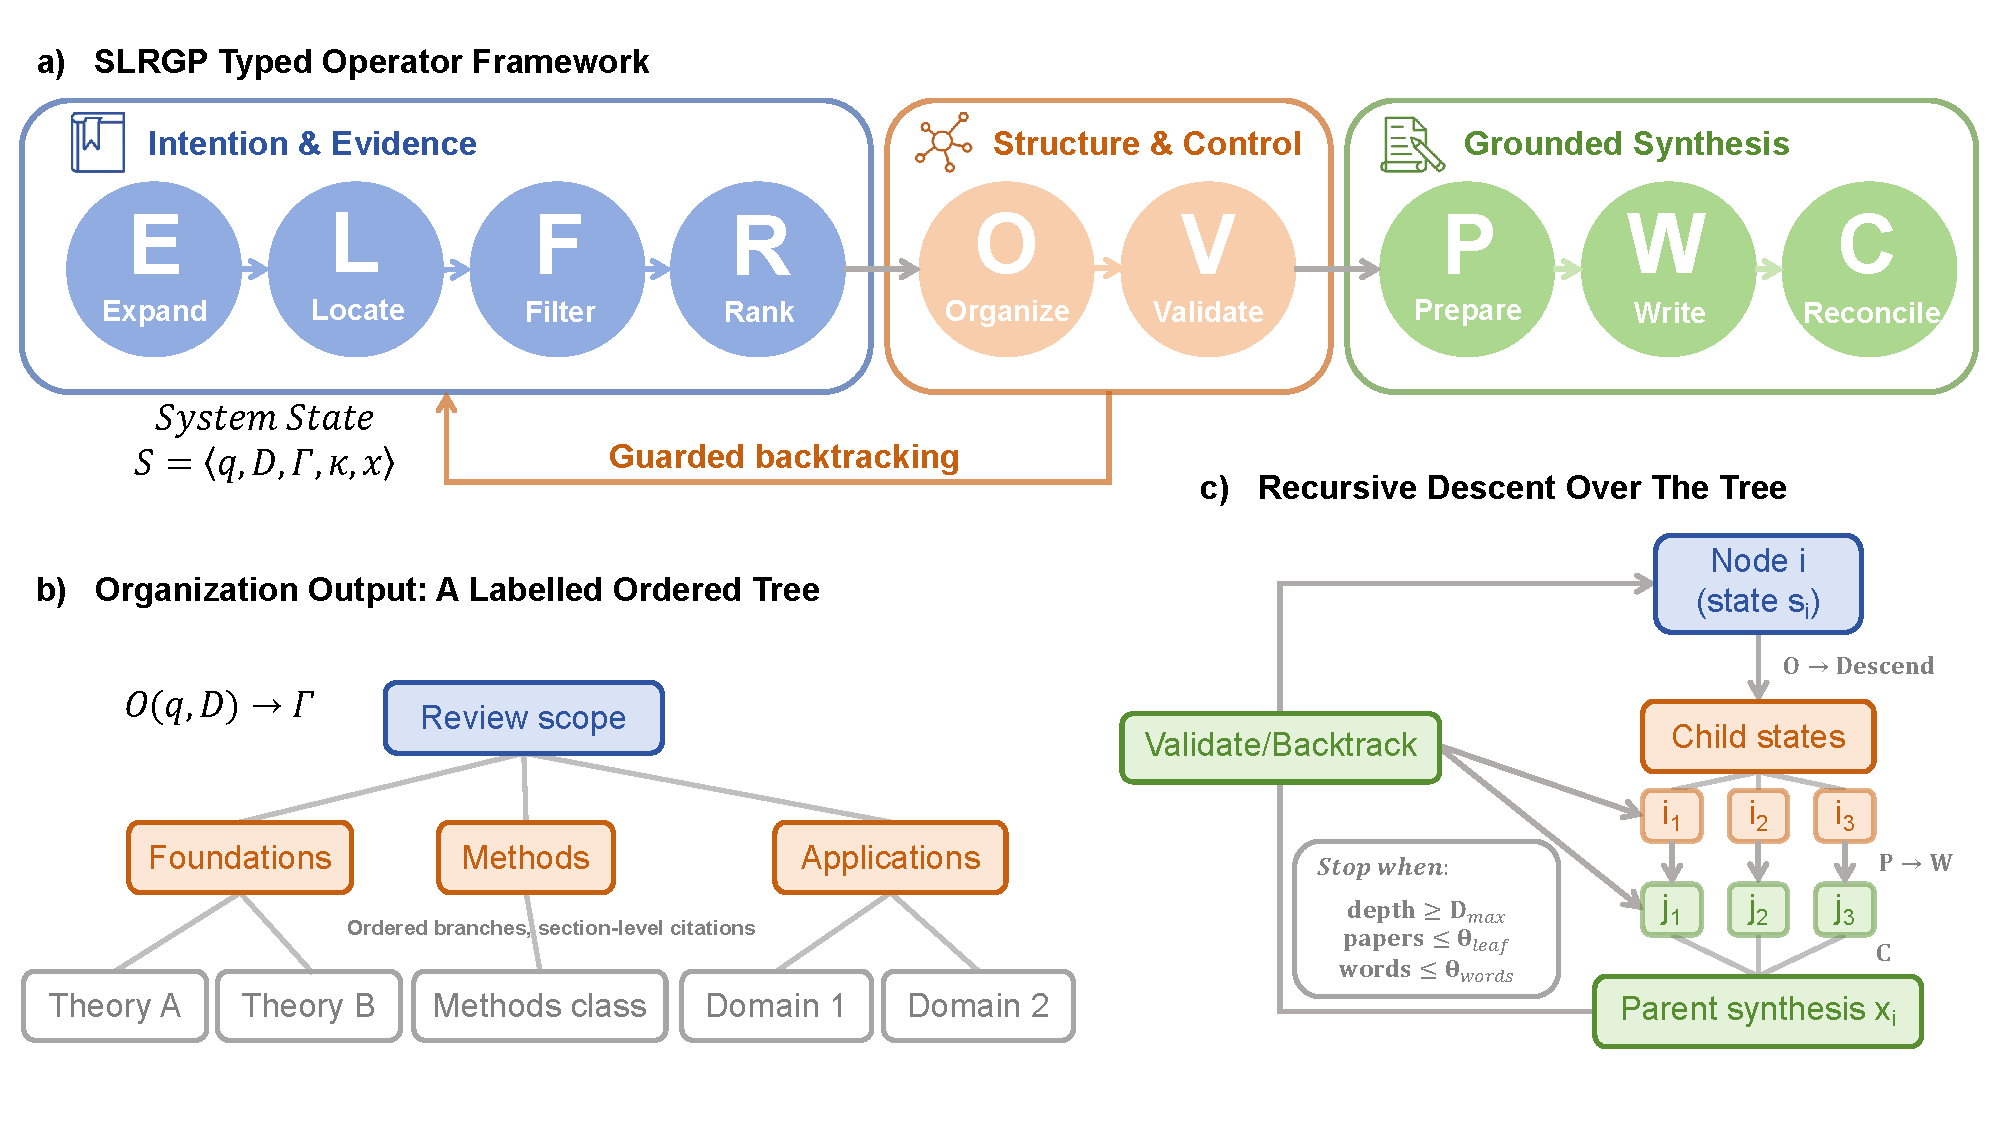
\includegraphics[width=0.85\linewidth,height=0.45\textheight,keepaspectratio]{figures/Figure1_operator_architecture.pdf}
\caption{\textbf{SLRGP formalizes literature-review construction as a typed, recursively composable operator system.} \textbf{a}, Nine operators transform a shared versioned state. \textbf{b}, $O$ represents organization as a LOTCF-LR (Labeled Ordered Tree Canonical Form for Literature Reviews) tree whose branches are labelled by a partition facet and ordering relation while retaining section-level evidence provenance. \textbf{c}, At an internal node, organization and descent induce child states; evidence preparation and bounded leaf writing occur locally, reconciliation merges child syntheses upward, and validation either accepts the result or backtracks. Recursion terminates at registered depth, evidence-count or word-allocation bounds.}
\label{fig:framework}
\end{figure}

This perspective also changes how automated-review research should be evaluated: end-to-end systems and isolated generation components can show whether plausible reviews are produced, but not which review-construction functions are required, which functions can be learned from observed review traces, or which failures arise when a function is weakened while its interface is held fixed. SLRGP therefore shifts the empirical question from ``can a system write a review?'' to ``can the logic of reviewing be structurally expressed, learned at its operator interfaces and recursively composed into higher-order synthesis?''


\section*{Results}

We evaluated SLRGP through five linked experiments that move from representational validity to practical deployment (Fig.~\ref{fig:design}): recovering organization from scholarly reviews, learning operator policies from citation and organization traces, measuring individual operators under matched substitutions, testing structural recursion beyond length scaling, and comparing the complete system with native external workflows. Each claim was tested against a matched control at the corresponding level, and confirmatory comparisons followed the frozen, blinded protocols described in Methods.

\begin{figure}[!t]
\vspace*{-2.2cm}
\centering
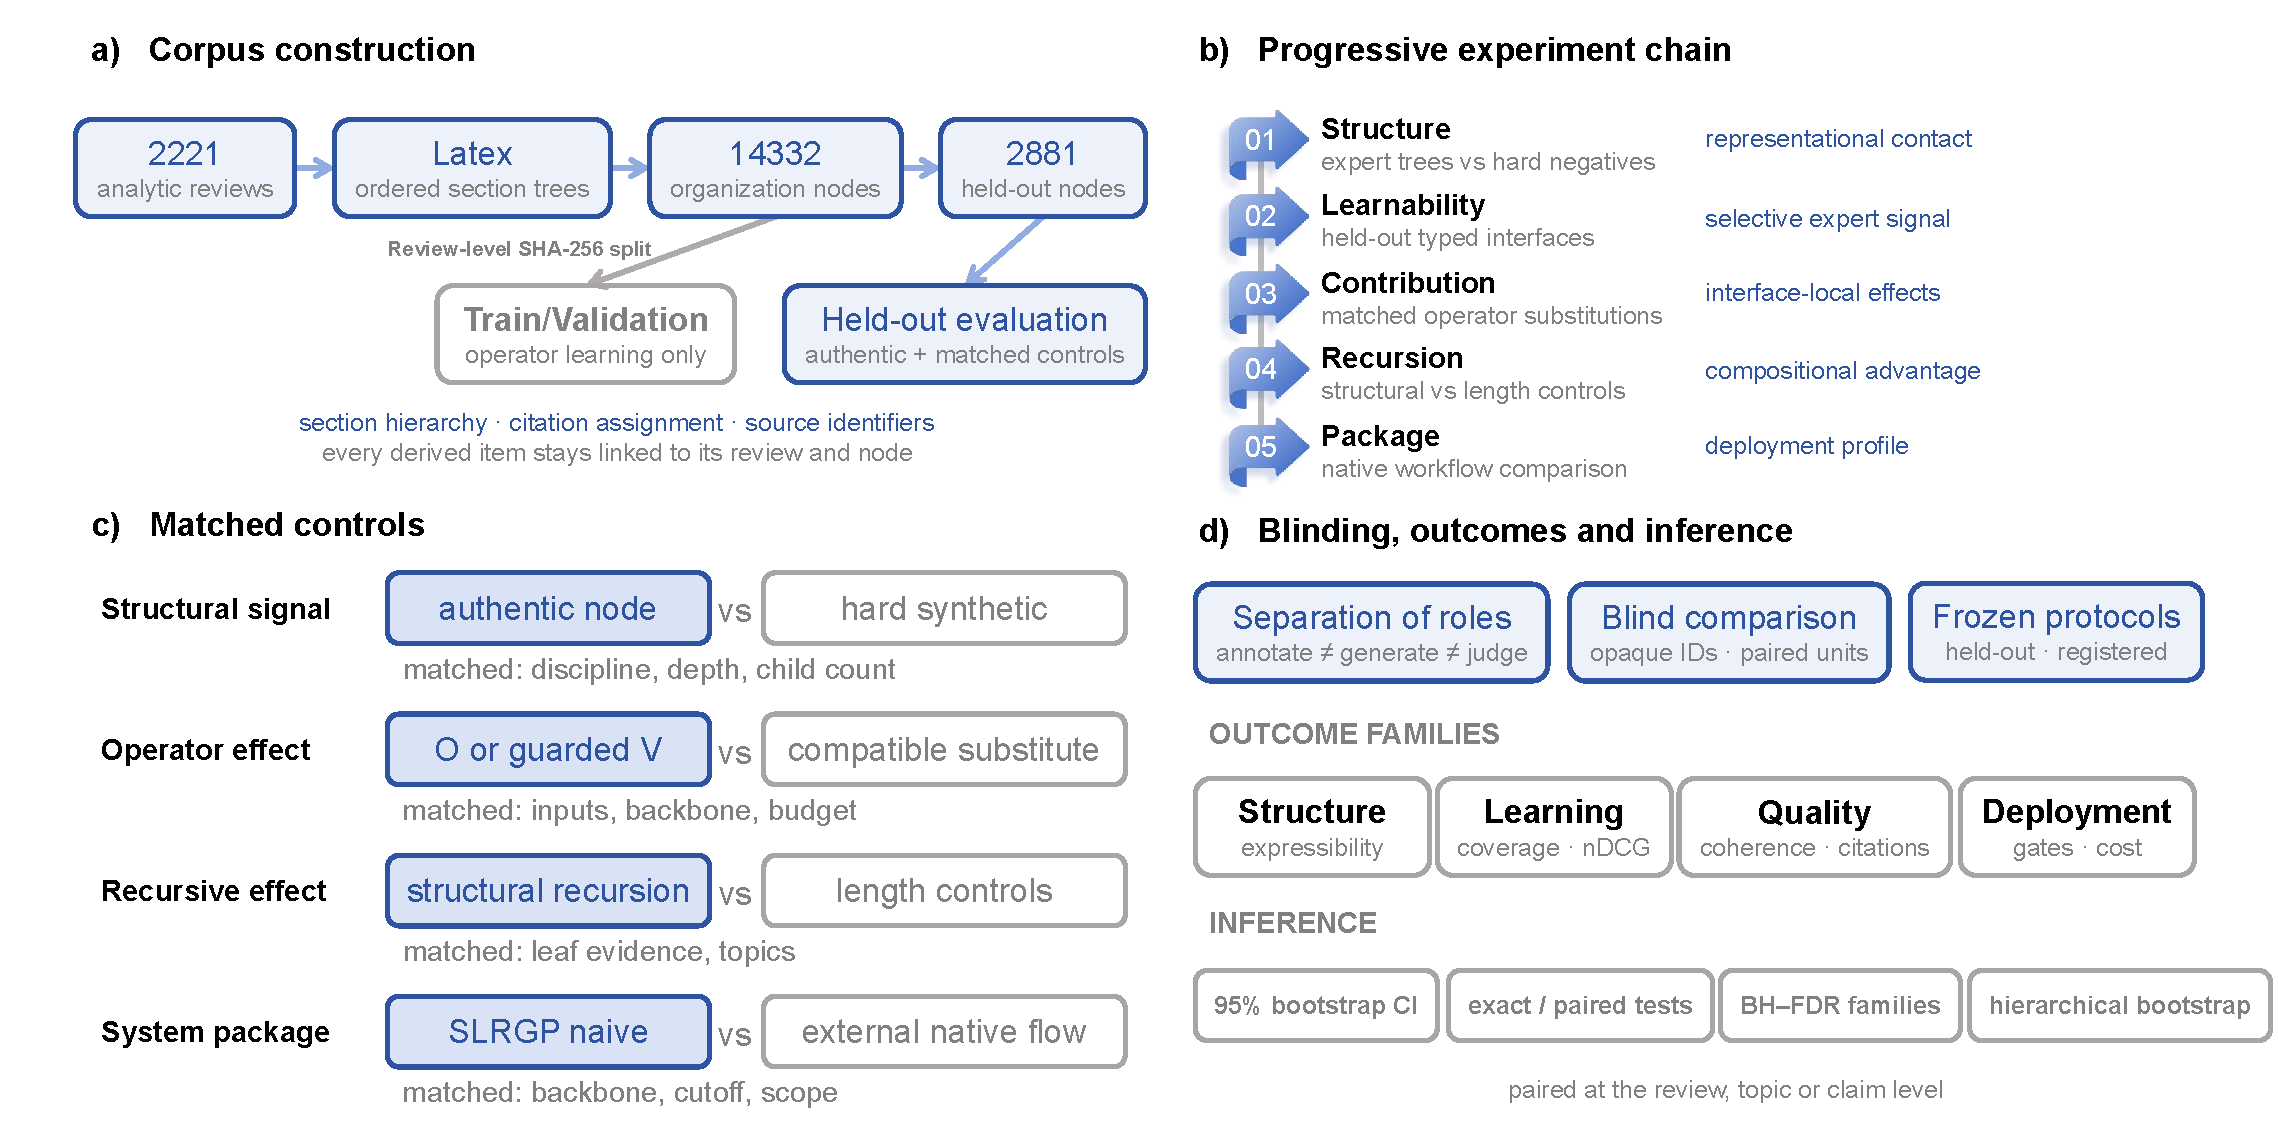
\includegraphics[width=0.95\linewidth,height=0.45\textheight,keepaspectratio]{figures/Figure2_experimental_design.pdf}
\caption{\textbf{Experimental design.} \textbf{a}, The corpus pipeline converts 2,221 arXiv reviews into ordered section trees with citation assignments, using review-level splits to separate operator learning from held-out evaluation. \textbf{b}, Five linked experiments move from structural recovery and operator learning to matched operator tests, recursive synthesis and native system comparison. \textbf{c}, Each claim is evaluated against a level-matched control while holding the relevant inputs, backbone, budget and scope fixed. \textbf{d}, Annotation, generation and judging are separated, while opaque identifiers, frozen protocols, paired tests and hierarchical resampling support blinded inference.BH--FDR, Benjamini--Hochberg false-discovery-rate correction.}
\label{fig:design}
\end{figure}

\FloatBarrier

\subsection*{1. SLRGP recovers the organizational structure of scholarly reviews}

We evaluated the representational adequacy of SLRGP by asking whether its reverse-parsing procedure could recover the organization of scholarly reviews as LOTCF-LR structures while preserving meaningful relations among sections and their evidence. Importantly, the experiment does not assume that the reviews were produced by SLRGP: it treats the manuscripts as observed products and tests whether SLRGP can structure them without reducing their organization to an arbitrary tree encoding. We applied the procedure to 2,221 scholarly arXiv review manuscripts across eleven disciplines whose LaTeX sources permitted deterministic recovery of section hierarchy and citation assignment (Supplementary Note~1).

The evaluation comprised two layers. The first tested \emph{structural recovery}: whether SLRGP could convert a review into an ordered section tree---the Labeled Ordered Tree Canonical Form for Literature Reviews (LOTCF-LR)---with section-level citation assignments. After a review-root node was added to canonicalize each top-level tree, the procedure recovered 14,332 organization nodes. Citation-child coverage was high (mean 0.935, median 1.0). This layer contains no language-model semantic judgement and establishes that SLRGP can recover the observable hierarchical and evidential structure of reviews in the analytic LaTeX population.

Structural recovery alone is insufficient because any table of contents can be encoded as a tree. The second layer therefore tested an operational measure of \emph{semantic fidelity}: whether the recovered representation retained organizing relations that distinguish authentic review structures from plausible counterfactual regroupings. We compared 2,881 held-out authentic nodes against hard matched counterfactuals constructed from discipline-matched donors with aligned depth and child-count structure. A single frozen annotation model (GPT-5.4-mini; see Methods) scored all samples under blinded conditions. Authentic and counterfactual structures were represented by opaque identifiers that did not reveal their condition (this frozen, model-based endpoint is not a substitute for independent human judgement; Supplementary Note~2).

Authentic structures received slightly higher scores than these hard negatives: the pairwise accuracy was 0.565, the ROC-AUC was 0.581 and the mean expressibility difference was 0.082 (95\% bootstrap CI [0.067, 0.096], permutation $p<10^{-4}$; Fig.~\ref{fig:evidence}a and Supplementary Table~1). The separation was small but consistently positive under matching for discipline, depth and child count. We therefore interpret it as a measurable organizational signal under the specified model-based endpoint, rather than as direct evidence of human cognitive equivalence; unmeasured lexical or construction cues may still contribute. This experiment establishes the first link in the evidence chain: the formal object used by SLRGP is recoverable from scholarly reviews and operationally distinguishable from matched alternatives.

\begin{table}[!b]
\caption{\textbf{Frontend-operator learnability and selected policies.}}
\label{tab:s2}
\centering
\small
\setlength{\tabcolsep}{5pt}
\renewcommand{\arraystretch}{1.08}
\begin{tabularx}{\linewidth}{@{}
  >{\raggedright\arraybackslash}p{3.10cm}
  >{\raggedright\arraybackslash}X
  >{\raggedright\arraybackslash}p{1.75cm}
@{}}
\toprule
\textbf{Operator} & \textbf{Held-out conclusion} & \textbf{Policy} \\
\midrule
\textbf{Expansion ($E$)} & No retrieval gain; ranking worsened & Default \\
\addlinespace[1.5pt]
\textbf{Location ($L$)} & Better allocation; recall remained limited & Hybrid \\
\addlinespace[1.5pt]
\textbf{Filtering ($F$)} & No gain over high-recall fusion & Default \\
\addlinespace[1.5pt]
\textbf{Ranking ($R$)} & Reranking improved candidate order & Learned \\
\addlinespace[1.5pt]
\textbf{Organization ($O$)} & Better partition and order prediction & Learned \\
\bottomrule
\end{tabularx}
\end{table}

\subsection*{2. Some frontend operators can be learned from scholarly review traces}

Second, we tested whether SLRGP could learn decision rules from observable traces in scholarly reviews, including citation choices and section organization. Each learning task was attached to an operator with clearly defined inputs and outputs. We focused on the five frontend operators that determine which evidence enters a review and how it is organized: expansion $E$, location $L$, filtering $F$, ranking $R$ and organization $O$. The other four operators have different roles and were not trained from these traces. Evidence preparation $P$, local synthesis $W$ and global reconciliation $C$ were implemented as controlled procedures that keep evidence traceable, preserve valid data structures and enforce length limits. Validation $V$ checks whether the proposed structure meets the required conditions and decides whether the system should retry with relaxed constraints. We evaluated this validation function by replacing it with a weaker alternative that had the same inputs and outputs, rather than by learning it from behavioural traces.

Learning did not improve every operator (Table~\ref{tab:s2}). Learned expansion $E$ did not increase retrieval coverage and reduced ranking quality when its expanded queries were passed to the downstream ranker. We therefore retained the default expansion policy (Supplementary Note~5). Learned location $L$ improved how candidates were allocated within the fixed top-300 budget. However, an audit of the first 3,000 retrieval results showed that roughly half of the papers cited in the source reviews were not found by either sparse or dense retrieval. Thus, $L$ could improve allocation among retrieved candidates, but it could not recover papers that were missing from the retrieved set (Supplementary Note~6 and Supplementary Table~2). Learned filtering $F$ showed some predictive signal when trained on eligibility labels produced by consensus among three models. These labels were only proxies, not a human-annotated gold standard, and the learned filter did not outperform the high-recall threshold based on reciprocal rank fusion\cite{rrf}. We therefore retained the default filtering policy (Supplementary Note~7).

Ranking $R$ and organization $O$, by contrast, showed clear and repeatable improvements after learning (Fig.~\ref{fig:evidence}b). The ranking model was trained on citation choices observed in the source reviews and used to reorder the top 300 candidates. It improved nDCG@10\cite{ndcg} by +0.153 over the baseline fusion order (95\% confidence interval [0.113, 0.201], $p\approx3\times10^{-10}$; Supplementary Note~8 and Supplementary Table~3). It also outperformed methods using only sparse retrieval, only dense retrieval, citation-aware scoring or linear pairwise ranking. Pre-registered leakage checks found no evidence of test-data leakage (Supplementary Note~8). The ranking advantage also remained in analyses that varied the assumed level of label noise. The main remaining constraint was retrieval recall: a ranker cannot reorder relevant papers that retrieval never placed in its candidate pool.

For organization, we described each observed organization decision with two labels: the criterion used to divide the literature and the relation used to order the resulting groups. A conservative logistic-regression model predicted held-out partition-criterion labels with an accuracy of 0.518, compared with 0.395 for a baseline using structural features alone (gain +0.110, 95\% CI [0.078, 0.141]). Its accuracy for ordering relations was 0.431, compared with 0.388 for the baseline (gain +0.038, 95\% CI [0.007, 0.069]). Prediction of the partition criterion remained stable across reviews of different lengths. Relation prediction was weaker because general-to-specific order and simple enumeration were often difficult to distinguish (Supplementary Note~4).

These findings show that learnability must be assessed separately for each operator. In the remaining experiments, we used the best validated policy for each one: default expansion and filtering, hybrid location, learned ranking and learned two-label organization.

\subsection*{3. Semantic organization and guarded validation independently improve quality}

Third, we tested whether semantic organization and guarded validation improve review quality independently of the language model that writes the text. Within a fixed pipeline, we replaced one operator at a time with a weaker alternative that accepted the same inputs and produced the same type of output. If review quality depended only on the language model's writing ability, these replacements should have had little effect. We kept the generation model, evidence pool, topic scope and source-tracking procedure unchanged.

All comparisons used the same initial evidence bundles, the same eight topics and a target length of 1,000 words. Organizing papers by meaning produced an overall quality score +0.417 higher than simply grouping consecutive papers by retrieval rank (95\% confidence interval [0.156, 0.729], exact $p=0.016$, false-discovery rate $q=0.047$; seven wins, no ties and one loss; Fig.~\ref{fig:evidence}c). Most of this gain appeared in organizational quality and global coherence, the two dimensions that the organization operator is designed to improve. Under deliberately introduced stress conditions, guarded validation increased quality by +0.375 across the six valid pairs (95\% CI [0.194, 0.569], $p=0.031$, $q=0.047$; six wins), after excluding two unguarded outputs below the required 850 words. Recursive descent, however, did not improve the matched short reviews ($\Delta=-0.021$, 95\% CI [$-0.135$, 0.083], $p=0.875$). We therefore tested the effect of recursion on longer reviews in the fourth experiment.

We repeated the two comparisons with positive results on four topics using a self-hosted, open-weight model. The direction of both effects remained the same in the valid comparison pairs. Overall, the replacement experiments show that semantic organization and guarded validation each contribute to quality within the tested pipeline (Supplementary Note~9 and Supplementary Table~4).

\begin{figure}[!b]
\centering
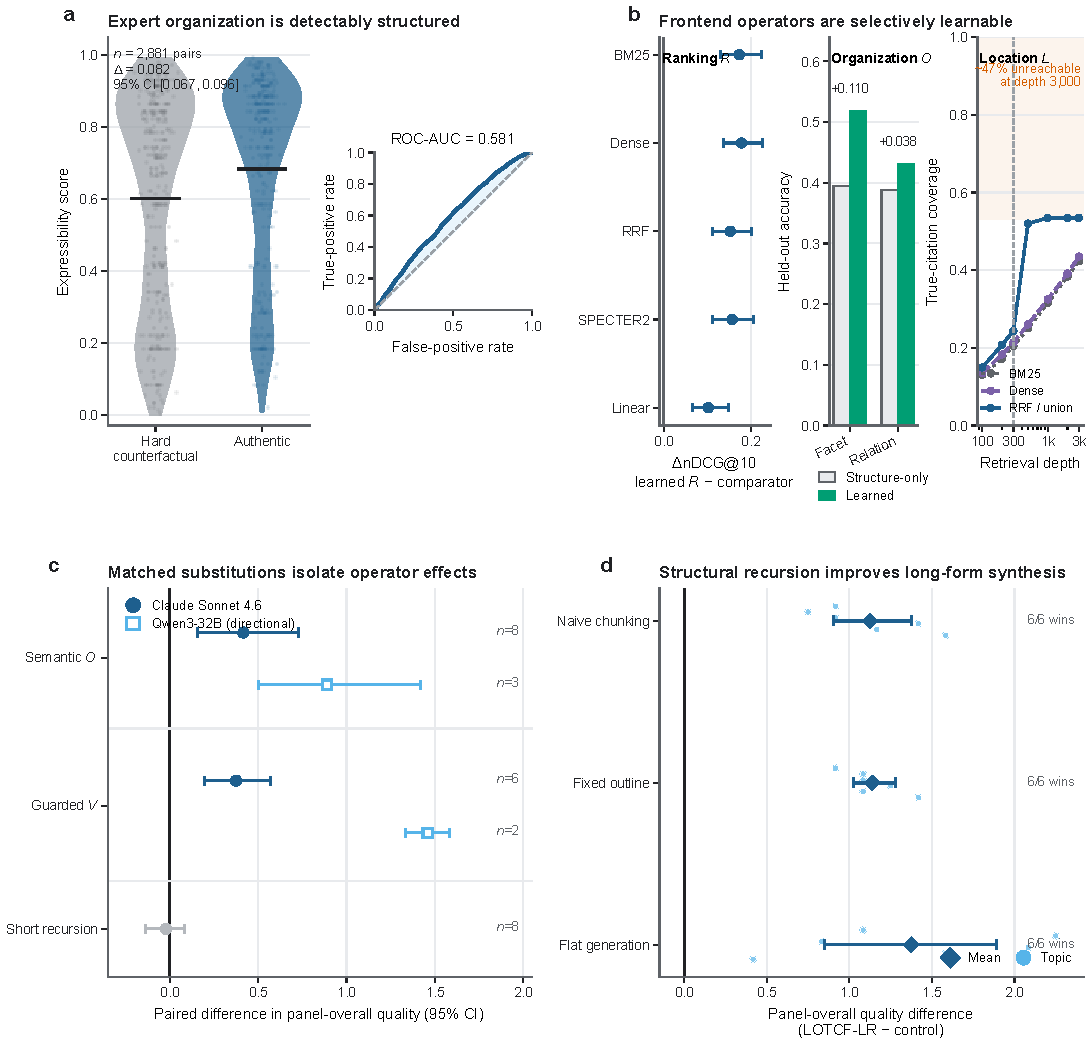
\includegraphics[width=0.85\linewidth,height=0.45\textheight,keepaspectratio]{figures/Figure3_internal_evidence.pdf}
\caption{\textbf{Evidence from the first four experiments.} \textbf{a}, Authentic review structures receive slightly higher scores than matched counterfactuals (mean difference 0.082). \textbf{b}, Learning improves ranking and organization, while retrieval recall limits the frontend. \textbf{c}, Semantic organization and guarded validation improve quality; short-form recursion shows no gain. \textbf{d}, Structural recursion outperforms naive chunking, fixed outlines and flat generation across all six long-form topics. Error bars show paired bootstrap 95\% CIs.}
\label{fig:evidence}
\end{figure}


\subsection*{4. Structural recursion improves long-form synthesis}

Fourth, we tested whether long reviews benefit from repeated organization at multiple levels, rather than from simply generating more words or splitting the evidence into chunks. In the tested implementation, SLRGP applied the organization operator again at each internal node of this hierarchy. It then wrote each leaf section from its local evidence within an assigned word limit and combined the completed sections from the bottom up. The evidence available to each child node was fixed to isolate the effect of structural recursion.

Stage A tested a system registered as \texttt{recursive\_slrgp}. In practice, this system only divided fixed evidence groups into adjacent writing units. It did not reorganize the material at internal nodes or combine child sections through the hierarchy. It did not reliably outperform flat generation or a fixed outline at the long target length. At the medium target length, its quality was lower than that of the fixed outline ($\Delta=-0.417$, $p=0.062$), and its difference from flat generation was not significant. A subsequent audit confirmed that this implementation performed chunking rather than the intended structural recursion (Supplementary Note~10 and Supplementary Table~5).

Stage B implemented the intended procedure as \texttt{structural\_\allowbreak lotcf\_\allowbreak recursive}. On the same six topics, the system selected a partition criterion and an ordering relation at every internal node, followed the resulting LOTCF-LR tree, wrote the leaf sections and merged them upward. Each output used the same fixed evidence pool and the same thirty-two leaf-level evidence cards as the three long-form controls. Structural recursion increased overall panel quality by +1.125 over naive chunking (95\% confidence interval [0.903, 1.375]), by +1.139 over a fixed outline ([1.028, 1.278]) and by +1.375 over flat generation ([0.847, 1.889]; Fig.~\ref{fig:evidence}d and Supplementary Table~6). All three comparisons had exact $p=0.031$, false-discovery rate $q=0.039$ and wins on all six topics. Organizational quality, global coherence and critical synthesis improved in every comparison. Citation plausibility was unchanged relative to naive chunking and the fixed outline. It was numerically higher than in flat generation, but the difference was not significant after correction ($\Delta=+1.000$, $q=0.072$).

The experiment therefore shows that, in this six-topic long-form setting, the quality gain came from organizing and combining evidence at multiple levels, not simply from splitting the evidence or assigning more words; this conclusion is based on matched leaf evidence and one randomized blind evaluation batch. Future experiments can test how the gain changes across target lengths and when child nodes retrieve additional evidence.



\subsection*{5. Native end-to-end comparison characterizes cost, quality and constraint compliance}

Finally, we compared the complete SLRGP system with AutoSurvey\cite{autosurvey}, SURVEYFORGE\cite{surveyforge} and SurveyGen\cite{surveygen}. All systems used the same generation model, publication cutoff and eight fixed topics, while retaining their own retrieval, organization and writing workflows. This experiment compares complete systems and therefore measures the combined effect of each workflow, not the effect of any single operator. It characterizes deployment under the tested native configurations rather than performance under a common system-level length controller (Supplementary Note~11).

The systems differed substantially in their ability to follow the output requirements (Table~\ref{tab:s3} and Fig.~\ref{fig:s3}). SLRGP was the only system that met both requirements---3,200--4,800 words and 40--60 references---for all eight topics. AutoSurvey and SURVEYFORGE met neither requirement on any topic and produced an average of 60,483 and 12,128 words, respectively. SurveyGen met the reference requirement on every topic but exceeded the length range on every topic, with a mean of 5,603 words.

\begin{table}[!htbp]
\caption{\textbf{Native end-to-end comparison on eight topics.} Gates are topics meeting the length/reference requirements. Preferences are probabilities of selecting SLRGP; parentheses give full-output BH--FDR $q$ values and exact $p$ values for 4,000-word excerpts. Cost is reported per output/per 1,000 words.}
\label{tab:s3}
\centering
\footnotesize
\setlength{\tabcolsep}{2.75pt}
\renewcommand{\arraystretch}{1.0}
\begin{tabular}{@{}lrccccc@{}}
\toprule
 & & & \multicolumn{2}{c}{Preference for SLRGP} & & \\[-10pt]
System & \shortstack{Mean\\words} & \shortstack{Gates\\L / R} & Full ($q$) & 4k ($p$) & \shortstack{Claim\\support} & \shortstack{Cost (\$)\\output / 1k} \\
\midrule
SLRGP & 4,032 & 8/8; 8/8 & --- & --- & 0.835 & 0.65 / 0.16 \\
AutoSurvey & 60,483 & 0/8; 0/8 & 0.312 (0.131) & 0.938 (0.0078) & 0.535 & 11.38 / 0.19 \\
SURVEYFORGE & 12,128 & 0/8; 0/8 & 0.948 (0.0156) & 1.000 (0.0078) & 0.559 & 7.46 / 0.62 \\
SurveyGen & 5,603 & 0/8; 8/8 & 0.354 (0.250) & 0.573 (0.633) & 0.707 & 3.01 / 0.54 \\
\bottomrule
\end{tabular}
\end{table}

\begin{figure}[!htbp]
\centering
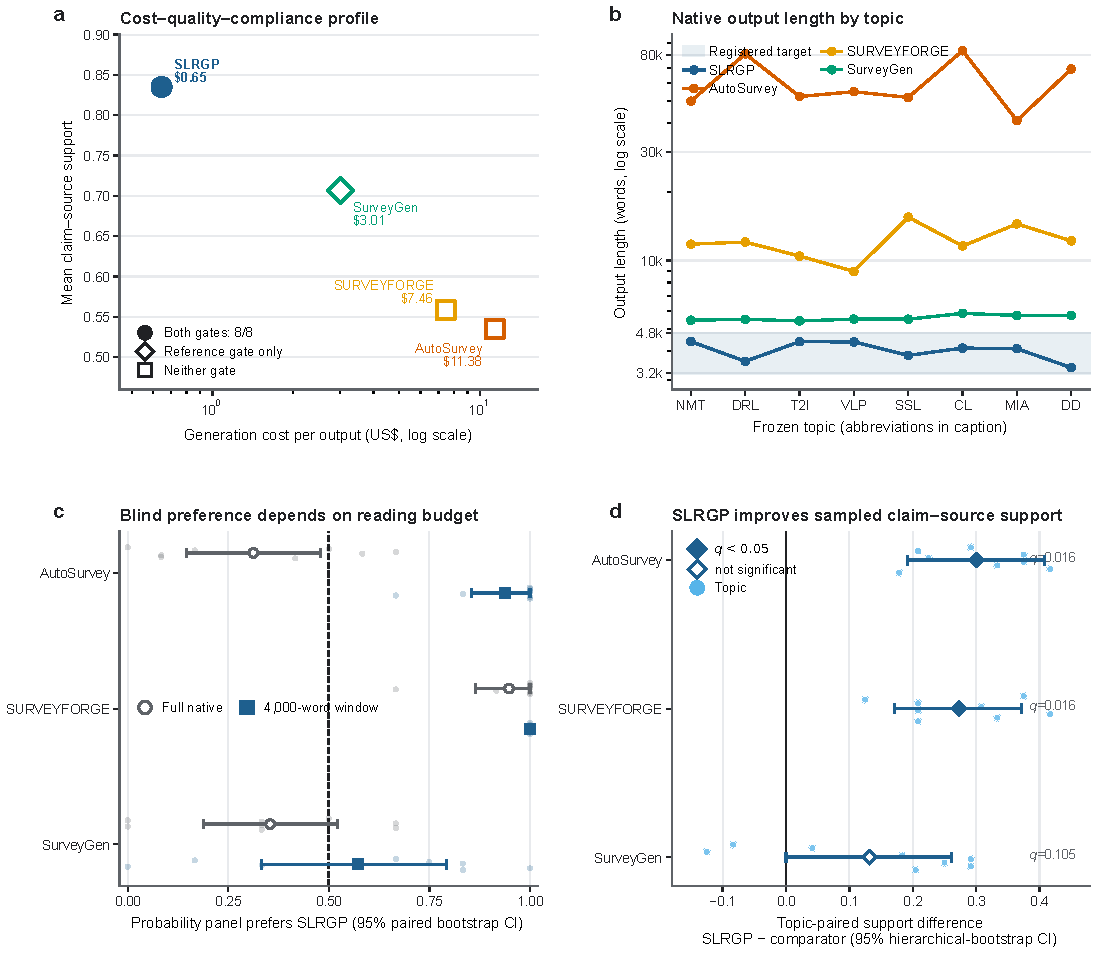
\includegraphics[width=0.85\linewidth,height=0.45\textheight,keepaspectratio]{figures/Figure4_native_comparison.pdf}
\caption{\textbf{Native end-to-end comparison of cost, quality and constraint compliance.} \textbf{a}, Per-output cost versus mean claim--source support; markers show constraint compliance. \textbf{b}, Topic-level output lengths against the 3,200--4,800-word target. \textbf{c}, Panel preference for SLRGP on full outputs and matched 4,000-word excerpts. \textbf{d}, Topic-paired differences in claim support with hierarchical-bootstrap 95\% CIs.}
\label{fig:s3}
\end{figure}


The preference results depended on whether the judges compared full outputs or equally sized excerpts. For the full outputs, the blinded three-model panel preferred SLRGP to SURVEYFORGE (preference probability 0.948, $q=0.0156$; eight wins), but did not prefer it to AutoSurvey (0.312, $q=0.131$) or SurveyGen (0.354, $q=0.250$). The result against AutoSurvey favoured AutoSurvey in direction but was not statistically significant. That comparison also required the panel to read outputs that differed by roughly fifteen-fold in length. We therefore performed the registered common-window analysis of 4,000-word excerpts: with reading length held constant, the panel preferred SLRGP to AutoSurvey (0.938, exact $p=0.0078$; eight wins) and SURVEYFORGE (1.000, $p=0.0078$; eight wins). The comparison with SurveyGen remained inconclusive (0.573, $p=0.6328$; five wins and three losses).

Following prior evaluations that distinguish citation presence from evidential support and factual precision \cite{alce,factscore}, we also checked whether cited sources actually supported the associated claims. For each output, we sampled twelve substantive claims that included citations. SLRGP obtained a mean support score of 0.835, compared with 0.535 for AutoSurvey, 0.559 for SURVEYFORGE and 0.707 for SurveyGen. In topic-paired comparisons, SLRGP scored +0.300 higher than AutoSurvey and +0.273 higher than SURVEYFORGE (both false-discovery rate $q=0.0156$). Its +0.132 advantage over SurveyGen was not significant after correction.

Generation cost was calculated from the recorded token counts using the official price of the shared generation model. The mean cost per output was \$0.65 for SLRGP, \$11.38 for AutoSurvey, \$7.46 for SURVEYFORGE and \$3.01 for SurveyGen. SLRGP used 28.8 total tokens per generated word, compared with 44.7 for AutoSurvey and 166--180 for the multi-pass SURVEYFORGE and SurveyGen. This corresponds to \$0.16, \$0.19 and \$0.54--\$0.62 per 1,000 generated words, respectively (Table~\ref{tab:s3}). The order-of-magnitude difference in their cost per completed output arose mainly because SLRGP met the required length, whereas AutoSurvey produced outputs that were about fifteen times longer.

Overall, SLRGP combined complete compliance with the output requirements, the highest observed mean claim-support score and the lowest per-output cost among the tested configurations. The comparison with SurveyGen was not statistically significant for either preference measure or for claim support, so these results should not be interpreted as universal superiority over every competing system.

\section*{Discussion}

This study treats automated literature reviewing as a sequence of explicit decisions, not only as the production of a final text. Across five experiments, we found that these decisions can be represented by operators with defined inputs and outputs, that some operator policies can be learned from observed citation and organization traces, and that recursive use of the operators improves long-form synthesis. When each system was tested with its original workflow, the complete SLRGP system also offered a favourable balance of quality, cost and compliance with output requirements.

The main design principle is the separation between an operator's role and the method used to implement it. An operator keeps the same input, output and responsibility whether it is implemented by a hand-written rule, a learned model or another auditable procedure. The learned ranker improved the order of retrieved papers, while its recall depended on the upstream candidate set. Likewise, both naive chunking and structural recursion created multiple writing units, but only structural recursion reorganized the material at several levels and merged the resulting sections through the hierarchy. The replacement experiments further showed that semantic organization and guarded validation made separate contributions when their inputs and outputs were held constant. This modular design also allows future language models to replace the current writing and reconciliation components without changing the rest of the system.

The external comparison establishes a descriptive result under the tested native configurations, not a controlled ranking under a common system-level length controller. SLRGP was the only tested system that met both the length and reference requirements for every topic. AutoSurvey produced an average of 60,483 words---about fifteen times the registered target---because its native workflow specifies a minimum length for each subsection. A future benchmark can complement this native-workflow comparison by applying a common total-length controller to every system. When the judges compared equally sized 4,000-word excerpts, they preferred SLRGP. Taken together, these findings show why deployable review systems should be evaluated for length and reference compliance as well as perceived quality.

Four directions follow directly from these results. First, future work can jointly train expansion with ranking and develop human-annotated eligibility sets for filtering. Second, the location operator can be extended with broader indexes, query portfolios and citation-graph retrieval to increase coverage before ranking. Third, structural recursion can be evaluated across additional target lengths while allowing each child node to perform its own expansion and retrieval. Fourth, independent domain experts can complement the blinded model panel and deterministic source checks.

The scope of inference is correspondingly bounded. The operator set is a task-derived construction framework rather than a unique or minimal model of human cognition; the structural-fidelity endpoint is model-based rather than human-validated; and the native comparison does not estimate performance under a shared system-level length controller. The six- and eight-topic experiments support paired effects in the tested settings, while broader topic generalization remains to be established. These boundaries motivate the human validation, controlled comparison and topic expansion described above.

The same approach may also help analyse other complex knowledge tasks, such as generating scientific hypotheses, analysing policy or conducting legal reasoning. Each task could be divided into functions that can be inspected, tested and combined recursively. More broadly, SLRGP provides a way to study scholarly synthesis through both its prose and the decisions that determine what evidence is selected, how it is organized and how the final argument is constructed.

\section*{Conclusion}

SLRGP frames literature reviewing as a composition of typed operators rather than an undifferentiated generation task. Across five experiments, the framework recovered scholarly review organization, supported learning at selected operator interfaces, isolated the contributions of semantic organization and guarded validation, and improved long-form synthesis through structural recursion. In the native end-to-end comparison, SLRGP also combined complete constraint compliance with strong observed sampled claim--source support and low per-output cost under the tested configurations, although its differences from SurveyGen were not significant. Together, these findings provide an inspectable empirical basis for building and testing literature-review systems.

\section*{Methods}

\subsection*{State representation and operator inputs and outputs}

SLRGP stores the current review as a versioned state $s=\langle q,D,\Gamma,\kappa,x\rangle$. Here, $q$ is the current review question, $D$ is the candidate literature set, $\Gamma$ is the organization tree, $\kappa$ records the result of validation and $x$ is the generated text. Each of the nine operators reads this state and may update only specified fields. Expansion $E$ and location $L$ refine the question and candidate set. Filtering $F$ and ranking $R$ remove or reorder candidates. Organization $O$ builds $\Gamma$ from the evidence and the selected organizational labels. Validation $V$ checks the tree and may send the system back to an earlier step. Preparation $P$ creates evidence cards for the tree, local synthesis $W$ writes a length-bounded section from those cards, and global reconciliation $C$ combines child sections and checks that citations remain attached to their supporting claims. Operators form a pipeline by passing this structured state from one step to the next. They form a hierarchy by applying the same operations recursively to the subproblems represented by nodes in $\Gamma$.

Formally, let $\mathcal{Q}$, $\mathcal{D}$, $\mathcal{G}$, $\mathcal{K}$ and $\mathcal{X}$ denote the types of the five persistent fields, so that $\mathcal{S}=\mathcal{Q}\times\mathcal{D}\times\mathcal{G}\times\mathcal{K}\times\mathcal{X}$. Evidence cards $a\in\mathcal{A}$ and registered budgets $b\in\mathcal{B}$ are typed auxiliary objects rather than persistent state fields: $P$ produces evidence cards for immediate use by $W$, while $b$ is read-only configuration. With $\mathcal{Q}^{+}$ denoting a finite query portfolio, $\mathcal{I}$ the retrieval index, $\Pi(\mathcal{D})$ an ordering of a candidate set and $\mathcal{X}^{*}$ an ordered family of child texts, the operator contracts are
\[
\begin{aligned}
E &: \mathcal{Q}\times\mathcal{B}\rightarrow\mathcal{Q}^{+},\\
L &: \mathcal{Q}^{+}\times\mathcal{I}\times\mathcal{B}\rightarrow\mathcal{D},\\
F &: \mathcal{Q}\times\mathcal{D}\times\mathcal{K}\rightarrow\mathcal{D},\\
R &: \mathcal{Q}\times\mathcal{D}\rightarrow\Pi(\mathcal{D}),\\
O &: \mathcal{Q}\times\mathcal{D}\times\mathcal{B}\rightarrow\mathcal{G},\\
V &: \mathcal{S}\times\mathcal{B}\rightarrow\mathcal{S}\times\{\mathrm{accept},\mathrm{retry},\mathrm{stop}\},\\
P &: \mathcal{D}\times\mathcal{G}\rightarrow\mathcal{A},\\
W &: \mathcal{Q}\times\mathcal{A}\times\mathcal{B}\rightarrow\mathcal{X},\\
C &: \mathcal{G}\times\mathcal{X}^{*}\times\mathcal{B}\rightarrow\mathcal{X}.
\end{aligned}
\]
These signatures specify interfaces rather than implementations. A composition is legal when the output type and registered preconditions of one operator satisfy the input contract of the next. Auxiliary outputs can be passed directly, as in $W(q,P(D,\Gamma),b)$, without extending the persistent state. Each implementation is lifted to a partial state transition $\widehat{f}:\mathcal{S}\rightharpoonup\mathcal{S}$ that may update only its declared fields. Valid transitions preserve evidence provenance, valid data structures and the attachment of citations to their supporting claims.

\subsection*{Guarded validation and termination}

Validation checks both mandatory requirements and quality-related preferences. Mandatory requirements include non-empty branches, complete citation links, traceable evidence sources and valid data structures. Quality preferences include balanced branches, an appropriate distribution of publication dates and adequate coverage. If a check fails, the system retries in a fixed order. It first broadens the query concepts, then relaxes eligibility criteria and finally retrieves additional evidence for the affected branch. Each step only enlarges the available evidence; it does not remove material that was already admissible. Execution stops when validation succeeds, when all relaxation steps have been used or when the configured iteration limit is reached.

Termination follows from the registered bounds rather than from an assumed fixed point. Along recursive descent, the remaining depth $D_{\max}-d$ strictly decreases; along guarded backtracking, the remaining retry allowance strictly decreases. Because each organization node has finitely many children and both quantities are bounded below by zero, every registered execution terminates.

\subsection*{Structural recursion}

At every internal node of $\Gamma$, \texttt{Descend} creates a child state with a more specific review question and a local set of evidence. In Stage B, we fixed the leaf-level evidence cards to isolate recursive organization, descent, length-bounded leaf writing and upward merging. Future extensions can activate expansion and retrieval within child states when local evidence is insufficient. Recursion stops when it reaches the maximum depth $D_{\max}$, when a node contains no more than $\theta_{\mathrm{leaf}}$ papers or when the words assigned to a node fall below $\theta_{\mathrm{words}}$. Sibling nodes are processed independently. Their outputs are then combined in the fixed order of the tree before a final consistency check.

\subsection*{Corpora}

The structural corpus contains 2,221 English-language scholarly arXiv review manuscripts from eleven disciplines. We use this term because arXiv availability does not itself imply peer review or independently verified expertise. We recovered section hierarchies and citation commands directly from the LaTeX sources using deterministic rules. Processing included expanding \texttt{\textbackslash input} and \texttt{\textbackslash include}, removing comments and identifying the main file. OpenAlex supplied bibliographic metadata and links between records referring to the same work\cite{openalex}. Supplementary Note 1 reports how many records could not be processed reliably and were excluded. The analytic population is therefore limited to manuscripts whose LaTeX sources support deterministic recovery. The corpus includes economics and quantitative finance, which we grouped as quantitative social sciences. We therefore repeated the semantic-expressibility analysis in this subset using the same registered held-out nested-node measure as in the main analysis (Supplementary Note 3).

\subsection*{Learned implementations of the operators}

Location $L$ combines sparse BM25 retrieval\cite{bm25} with dense retrieval by reciprocal rank fusion\cite{rrf}. Its learned allocation policy changes the relative weight of these signals while keeping the candidate budget fixed at 300. Ranking $R$ uses a LambdaMART-style gradient-boosted tree model\cite{lambdamart,lightgbm} trained on the papers cited in the source reviews. Reviews, rather than individual papers, were assigned to separate data splits. We also included checks for data leakage and tested whether the results were sensitive to noisy labels. Organization $O$ uses logistic regression to predict the partition criterion and ordering relation, with a model based only on structural features as the baseline. All learned models were fixed before confirmatory evaluation began.

\subsection*{Experimental design}

The structural experiment had two parts. First, deterministic rules recovered labelled and ordered section trees and assigned citations to sections. Second, a single annotation model (GPT-5.4-mini) scored authentic structures and closely matched counterfactual alternatives without knowing which was which. The model was fixed before evaluation. All structures were shown with random identifiers generated within each batch, and these identifiers revealed nothing about the experimental condition. This endpoint operationalizes organizational fidelity for the present analysis; independent human scores can provide a separate validation while retaining the same blinded identifiers and frozen comparison set.

The learnability experiments split data at the review level using SHA-256 hashes. Organization learning used an 80/20 split, whereas ranking used 70/15/15 splits. Test-set scoring began only after the code was fixed.

The operator-replacement experiment used Claude Sonnet 4.6, eight topics and a target length of 1,000 words. It replaced one operator at a time with an alternative that had the same interface, while keeping the rest of the source-tracking pipeline fixed. We repeated the two comparisons with positive results on four topics using Qwen3-32B to check whether the direction of the effects was preserved.

The long-form experiment had two stages. Stage A compared naive chunking, a fixed outline and flat generation at three target lengths. Stage B tested the full structural sequence $O\rightarrow\text{Descend}\rightarrow\text{leaf}\rightarrow\text{Merge}$ at the long target length, using matched evidence at the leaf nodes.

The end-to-end comparison ran the original workflows of SLRGP, AutoSurvey\cite{autosurvey}, SURVEYFORGE\cite{surveyforge} and SurveyGen\cite{surveygen}. All used Claude Sonnet 4.6, a 2023 publication cutoff and the same eight topics. A blinded panel of three different models evaluated both the complete outputs and registered excerpts of 4,000 words. Each pair was presented in two randomized orders, and a tie received a score of 0.5. The released AutoSurvey interface specifies a minimum length for each subsection, so we preserved this native setting and report the resulting output lengths. A future tuned comparison can additionally impose a common total-length controller across all systems.

\subsection*{Evaluation panel and validation}

LLM-based judges can provide scalable preference measurements, but prior work has identified position, verbosity and self-preference effects; cross-family panels have been proposed as one way to reduce dependence on any single evaluator \cite{llmjudge,selfpreference,poll}. Panel J therefore consists of three blinded evaluators from different model families: GPT-5.5, Gemini 3.1 Pro Preview and Claude Sonnet 5. System names were removed from the outputs, and presentation order was randomized. The panel scored four dimensions: organizational quality, critical synthesis, citation plausibility and global coherence. To check that the panel could detect known defects, we used two published full-length reviews under eight conditions. Each of the three evaluators scored every condition twice, producing 96 valid calls out of 96. Reordering sections or replacing citations with shuffled alternatives significantly reduced the scores, showing that the panel responded to structural and citation errors (Supplementary Note~12 and Supplementary Table~7).

\subsection*{Statistics}

All primary comparisons pair observations by topic or by review. In the topic-based experiments, topics are the unit of inference. Pairing reduces between-topic variation, and exact tests are used because the topic counts are too small for reliable asymptotic inference. Depending on the analysis, we report bootstrap confidence intervals, exact tests or Wilcoxon paired tests, together with paired effect sizes and win/tie/loss counts. Within each pre-specified family of comparisons, we control the false-discovery rate using the Benjamini--Hochberg procedure\cite{benjamini1995}. Retrieval queries with no positive examples remain in the main ranking analysis and receive a score of zero. For claim-support analysis, hierarchical bootstrap resampling follows the order topic $\rightarrow$ output $\rightarrow$ claim. Robustness checks registered as directional tests report whether the effect points in the same direction and how it changes under alternative analysis choices; they are not presented as new confirmatory significance tests.

\FloatBarrier

\noindent\textbf{Code and data availability.} The corpus provenance manifests, learned-operator code, generation and evaluation pipelines, and all confirmatory outputs, traces and judgment logs referenced in this study accompany this submission as a code-and-data package and are publicly available at \url{https://github.com/amark071/SLRGP}.

\noindent\textbf{Competing interests.} H.W. is the founder of Beijing Liaoyuan Shuke Information Technology Co., Ltd., which is developing commercial products related to this work. Q.L. is an employee of Trueland Information Technology (Shanghai) Co., Ltd. The remaining authors declare no competing interests.

\noindent\textbf{Author contributions.} H.W. conceived the framework, designed the study and experiments, and led the writing. Y.Z. contributed to the mathematical formalism. Y.D. supervised the research and critically revised the manuscript. T.H. contributed to the experimental design and to the review of the manuscript. Q.L. contributed to data engineering and system implementation. All authors reviewed and approved the final manuscript.
\bibliographystyle{naturemag}
\bibliography{references}

\end{document}
